\documentclass{article}
\usepackage{graphicx} % Required for inserting images
\usepackage{amsmath}
\usepackage{amssymb}
\usepackage{caption}
\usepackage{indentfirst}
\usepackage{float}
\usepackage[a4paper, total={6in, 10in}]{geometry}

\title{Mathcamp 2026 Qualifying Quiz Problem 6 Solution}
\author{Applicant ID: 25107}
\date{}

\begin{document}
	
	\maketitle
	
	Consider the directed graph $G$ formed by each mentor's guess, where an edge from node $u$ to node $v$ means that mentor $u$ guessed mentor $v$. This graph has $15$ nodes and $15$ edges, with each node having outward degree $1$. 
    
    Let $G'$ be the undirected graph of $G$, that is, its edges connect the same nodes in $G$ but are undirected. Denote two vertices in $G'$ to be \textit{connected} if there is a set of edges in $G'$ that form a path between those two vertices. A \textit{connected component} in $G'$ is a connected subgraph whose vertices are not a subset of any larger connected subgraph. Call the corresponding subgraph in $G$ a \textit{weakly connected component}. As there are no edges between two weakly connected components, we can consider them individually.
\begin{figure}[h]
    \centering
    \vspace{-0.3cm}
    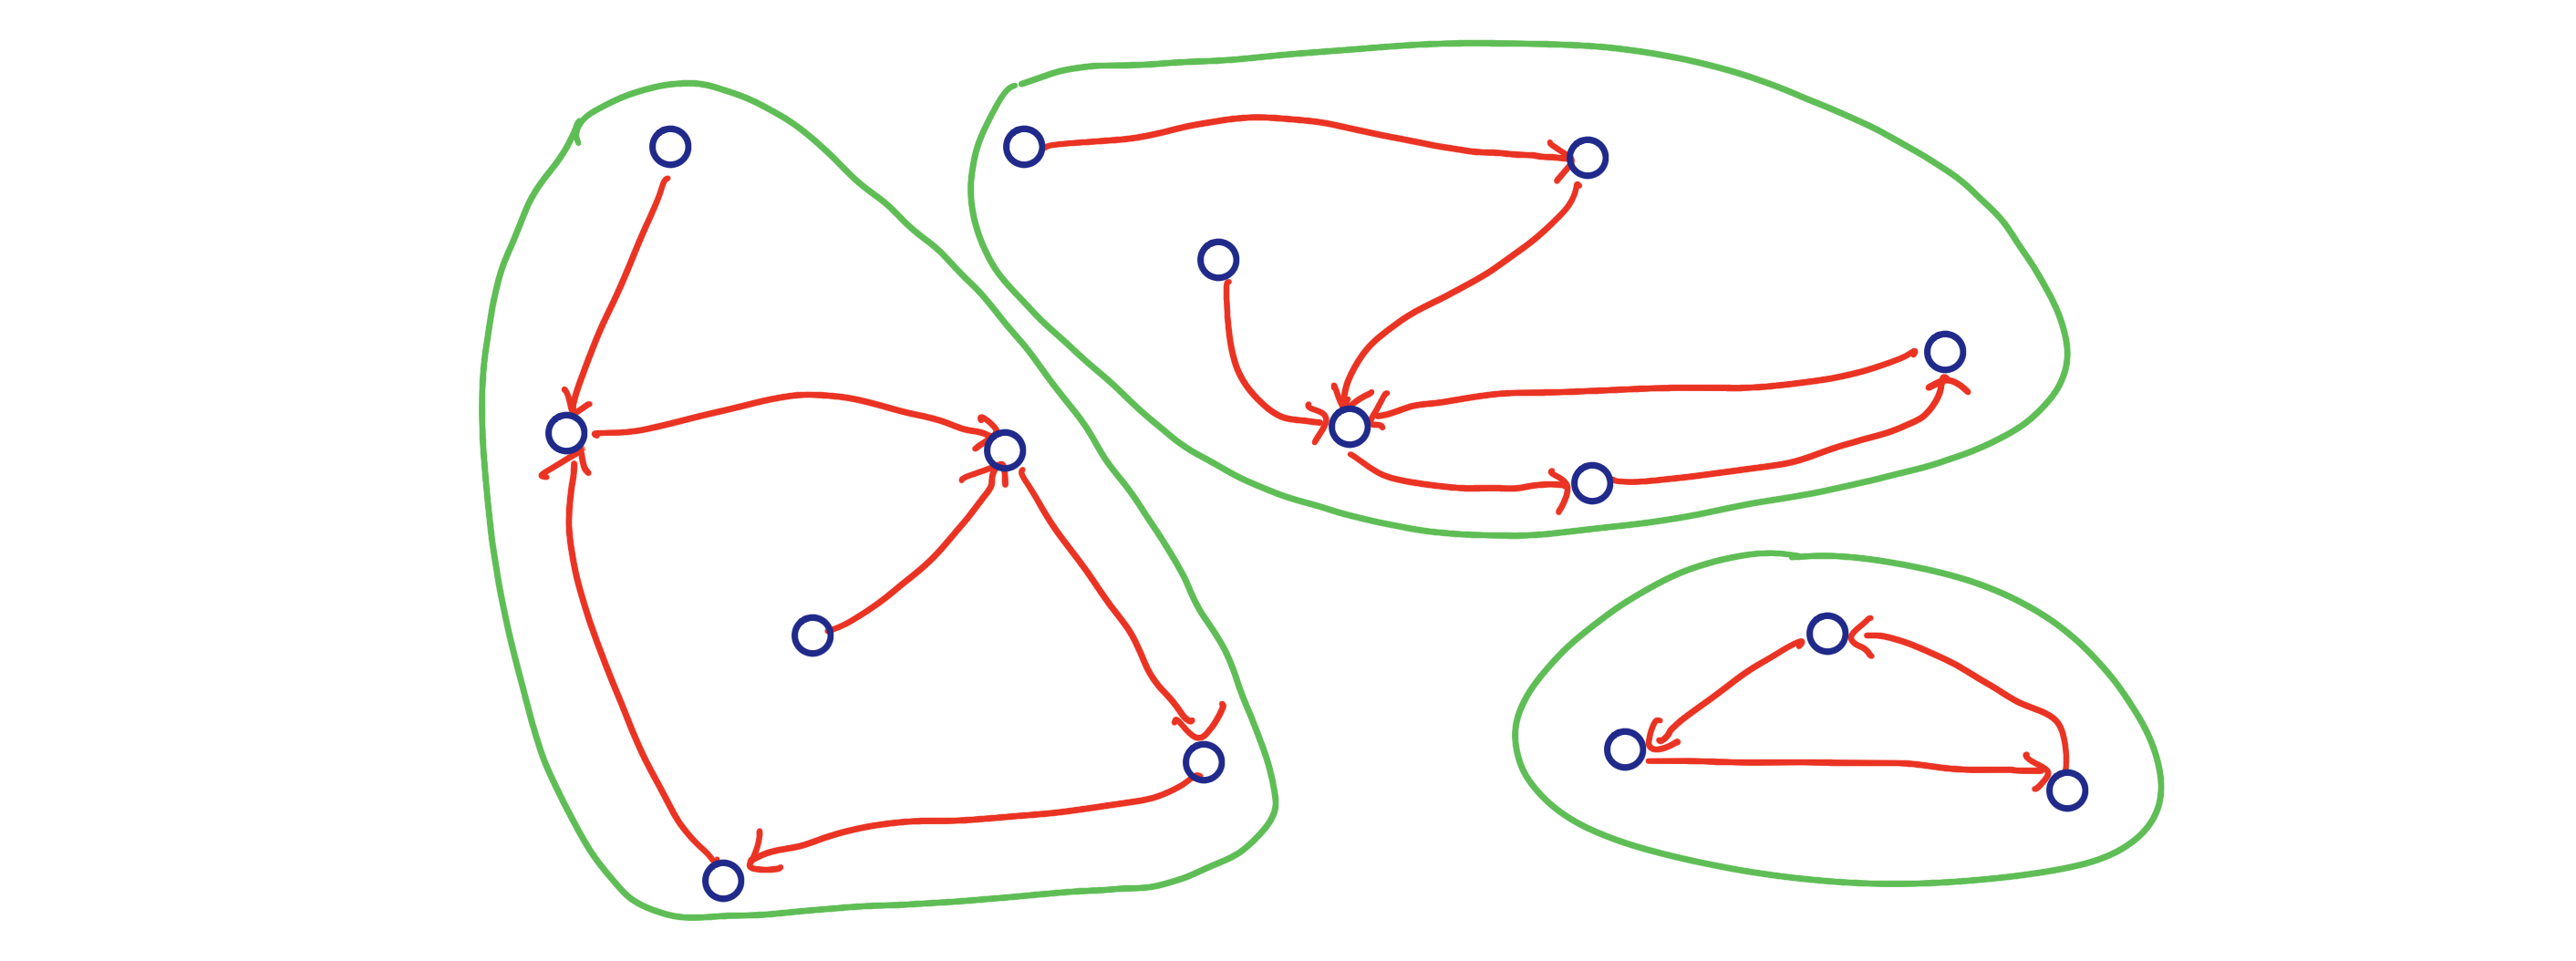
\includegraphics[width=14cm]{component.png}
    \vspace{-0.3cm}
    \caption*{A graph divided into weakly connected components (green)}
\end{figure}

    First, we show that each weakly connected component contains a cycle (a path of edges where the first and last vertices are equal). Let the component contain $n$ vertices. Start from any vertex $v_1$, and let the list $v_1, v_2, \dots, v_{n + 1}$ be the vertices reached while repeatedly traversing outgoing edges $n$ times. By the Pigeonhole Principle, as there are only $n$ distinct vertices, there must exist $i < j$ such that $v_i = v_j$, which means that the vertices $v_i, v_{i + 1}, \dots, v_{j - 1}$ form a cycle.

    Next, we show that each weakly connected component contains exactly one cycle. If a component has has $n$ vertices, it has $n$ edges. Consider the operation that transforms each cycle into a single vertex. The resulting graph is connected, and we claim that there are no new resulting cycles. This is because each vertex has outdegree 1, so it cannot be part of multiple distinct cycles. Therefore, the resulting graph must be a tree, i.e. with $m$ vertices and $m - 1$ edges. Suppose the original graph contained $c$ cycles. If a cycle has $k$ vertices, after being contracted by our operation to a single vertex, $k - 1$ vertices and $k$ edges are removed. Therefore, the resulting graph must have $c$ less edges than vertices. Hence $c = 1$, and each weakly connected component has exactly 1 cycle.
\begin{figure}[H]
    \centering
    \vspace{-0.3cm}
    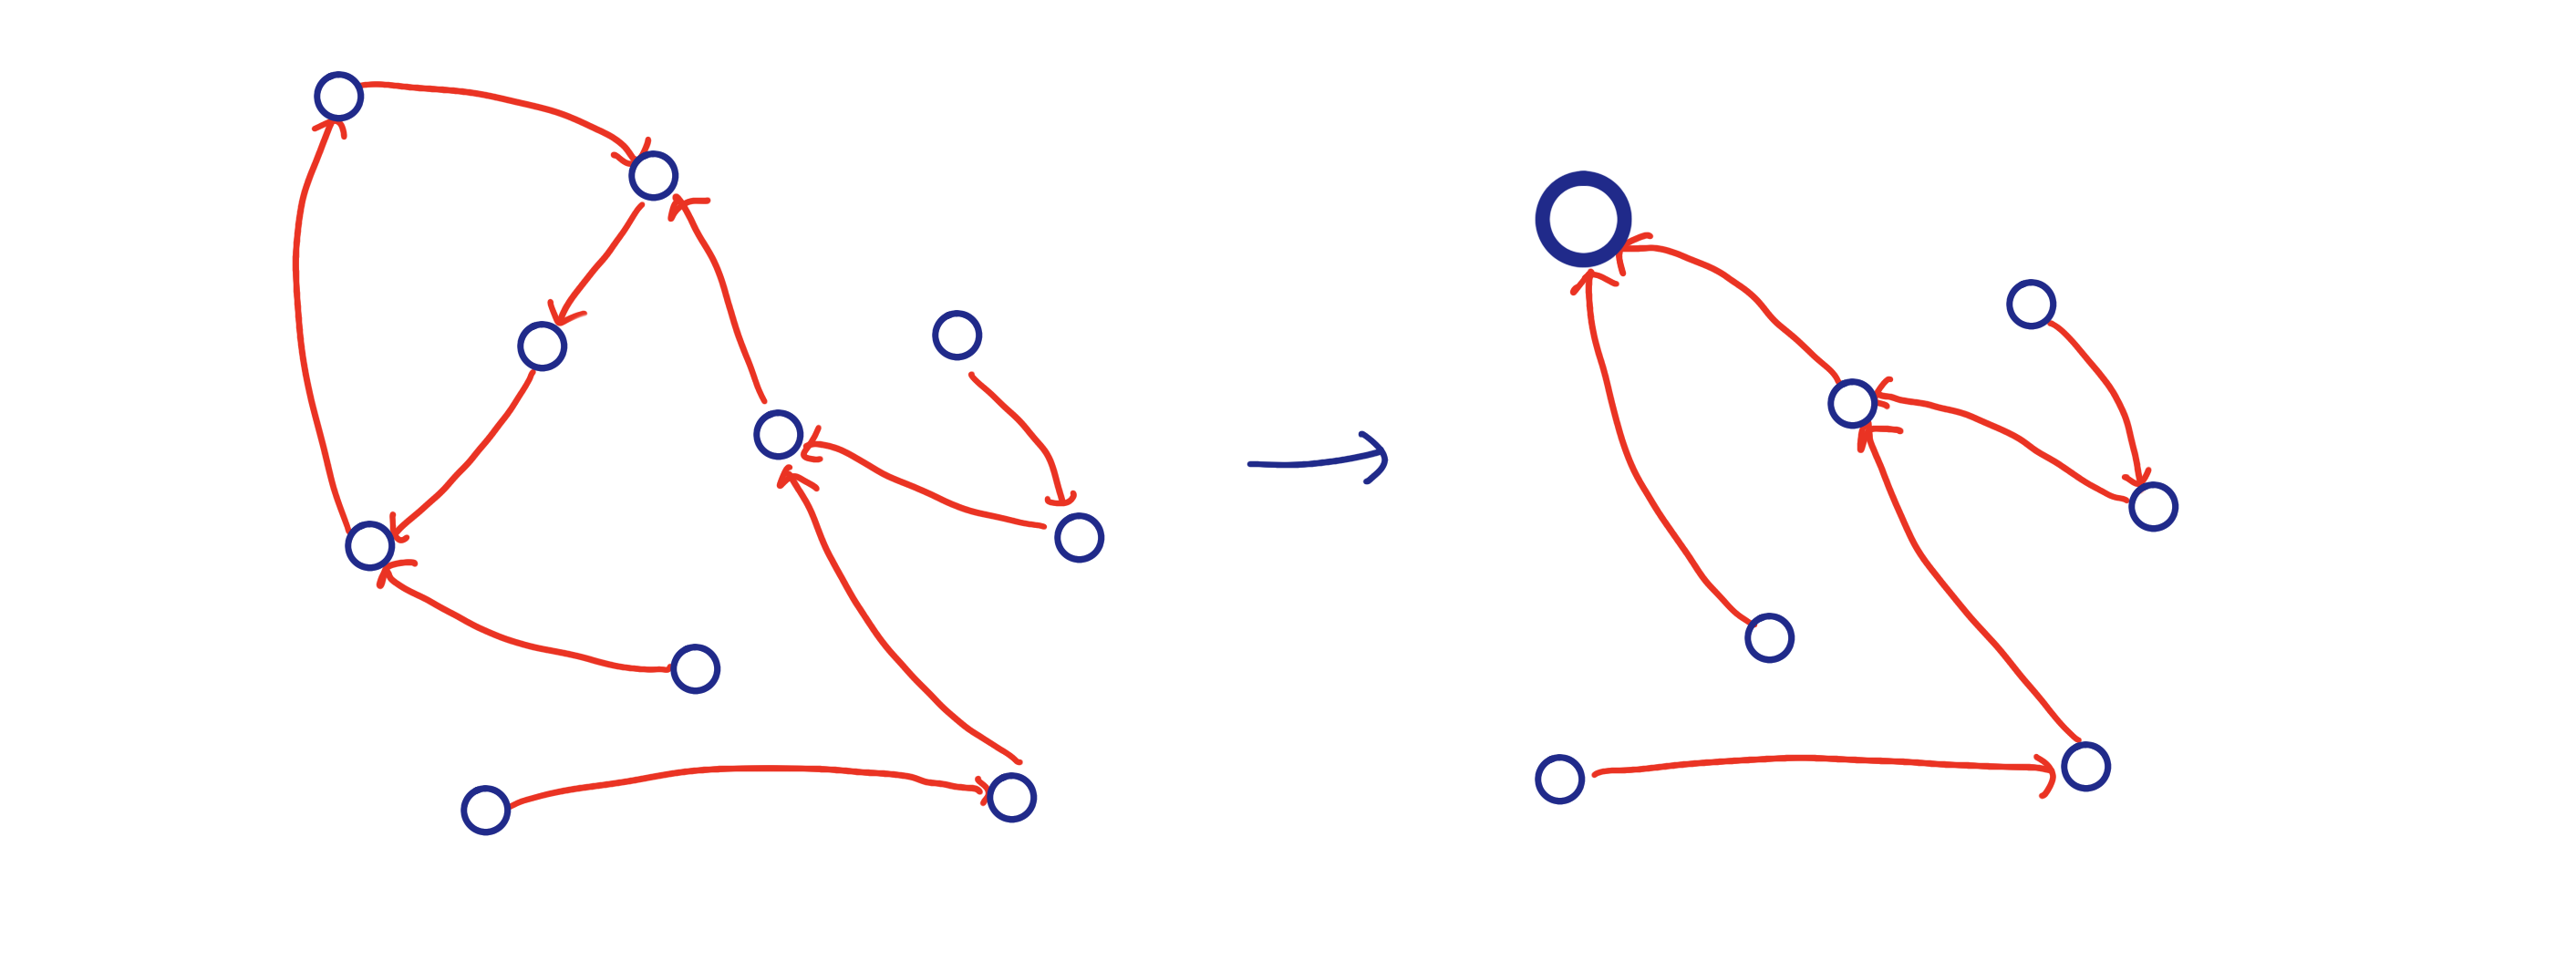
\includegraphics[width=14cm]{shrink.png}
    \vspace{-0.3cm}
    \caption*{Transforming a cycle into a vertex}
\end{figure}

    Finally, we consider the worst case scenario for the connected component, by assigning cookie types to each node. First notice that we can ignore the direction of the edges: all that matters is whether the two cookie types connected by that edge match. It is well known that trees are bipartite, that is, we can assign each vertex to one of two sets such that any two vertices connected by an edge are in different sets. So, if a vertex in the cycle is assigned a cookie type, we can assign cookie types to all vertices in its subtree (vertices that can be reached without traversing the cycle) such that no edge connects two vertices with the same type. So, no boxes of cookies can be kept by vertices in that subtree.
\begin{figure}[h]
    \centering
    \vspace{-0.3cm}
    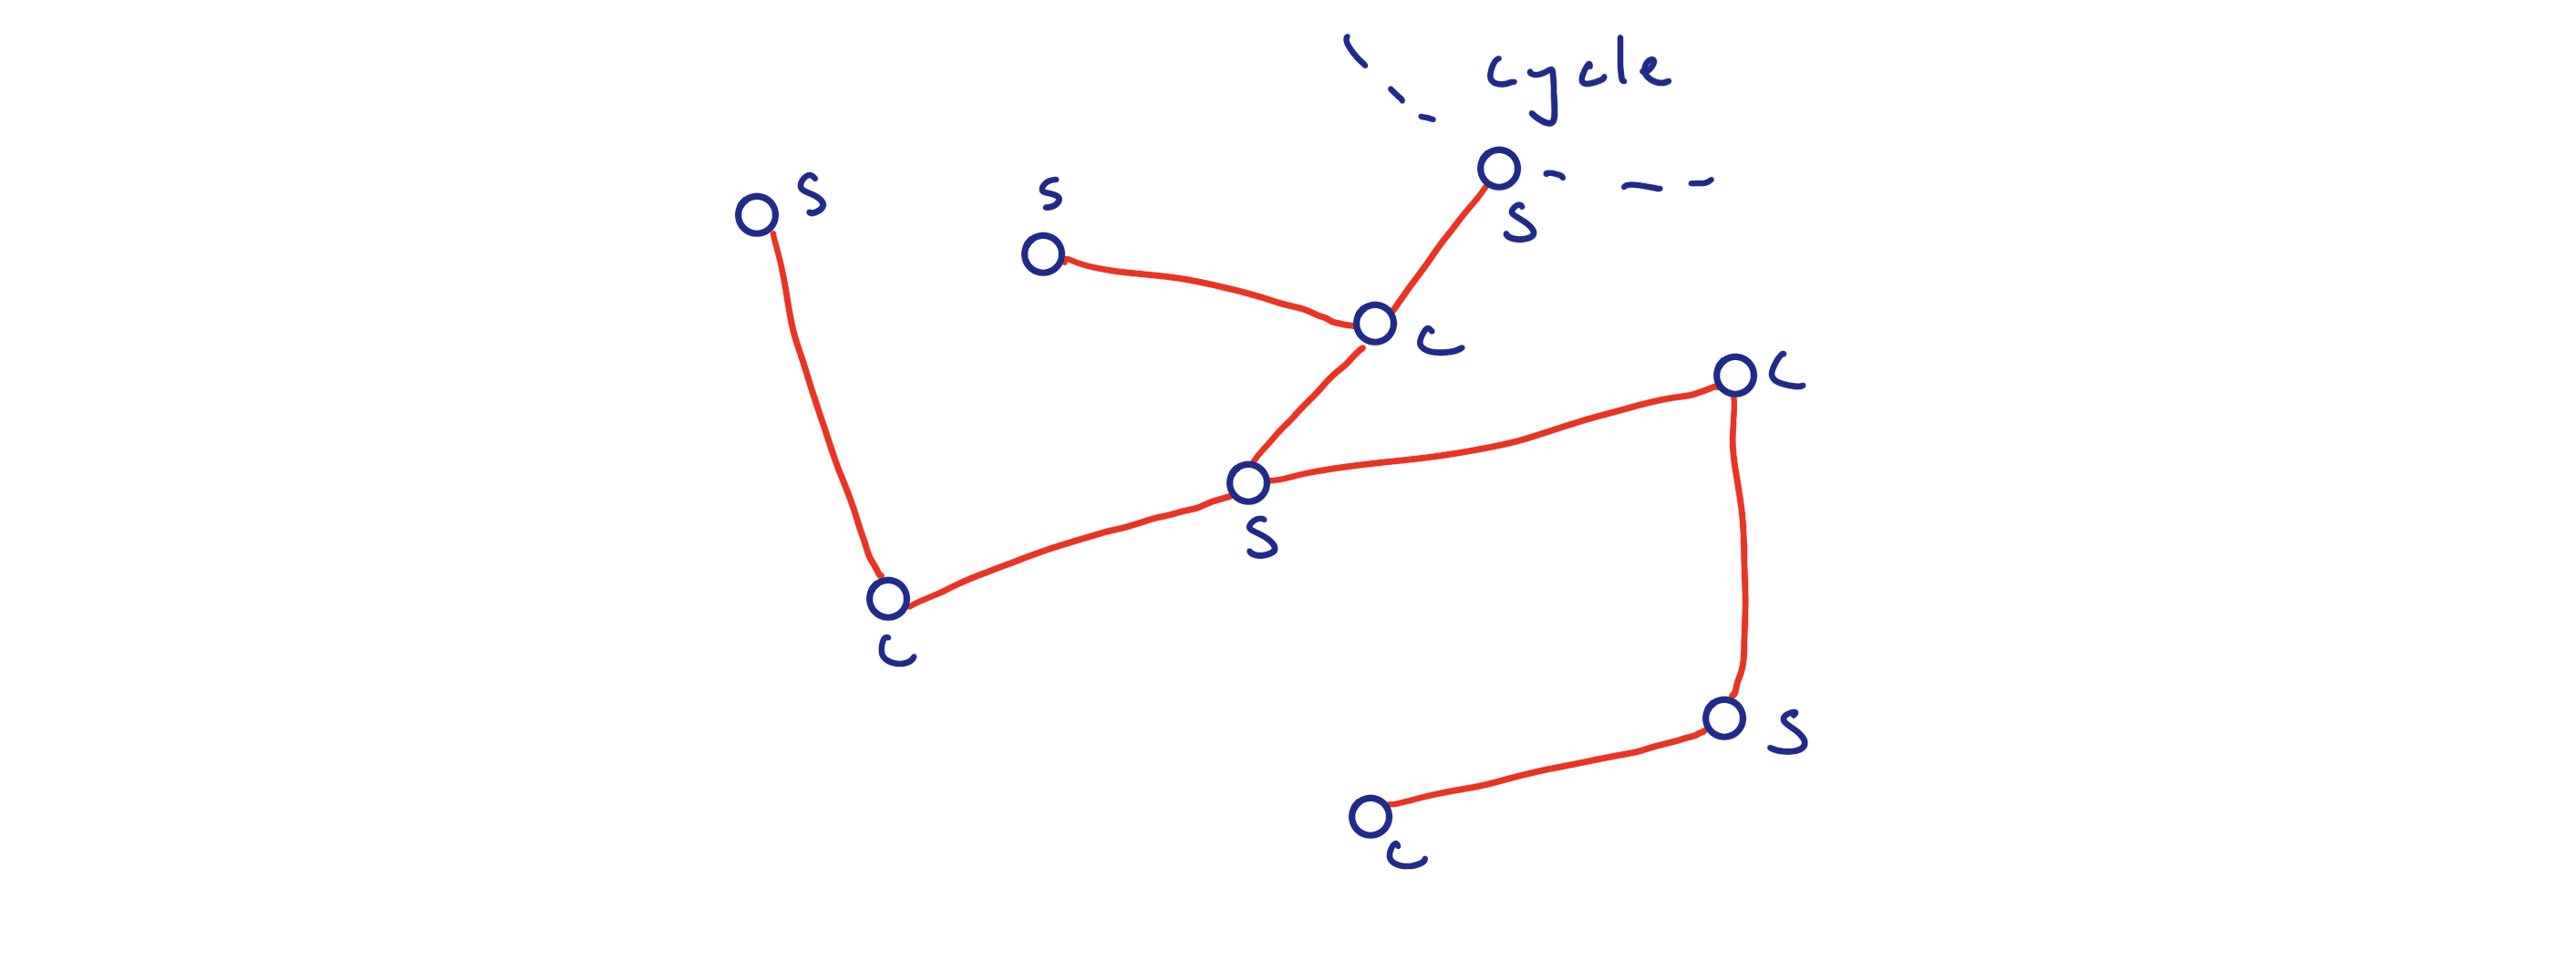
\includegraphics[width=14cm]{tree.png}
    \vspace{-0.3cm}
    \caption*{Bipartite coloring of a tree}
\end{figure}

    Now all that remains is the cycle. Clearly, if the cycle has even length, by alternating cookie types there will be no edges that connect vertices with the same type. However, this is not the case for odd cycles, where there must be at least one edge that connects vertices with the same type, therefore guaranteeing a box of cookies for the weakly connected component. From this, we see that the optimal strategy is to maximize the number of components with odd-length cycles. The smallest odd-length cycle contains $3$ vertices, so with 15 mentors, we can create 5 cycles and therefore guarantee to keep 5 boxes of cookies.    
\begin{figure}[h]
    \centering
    \vspace{-0.3cm}
    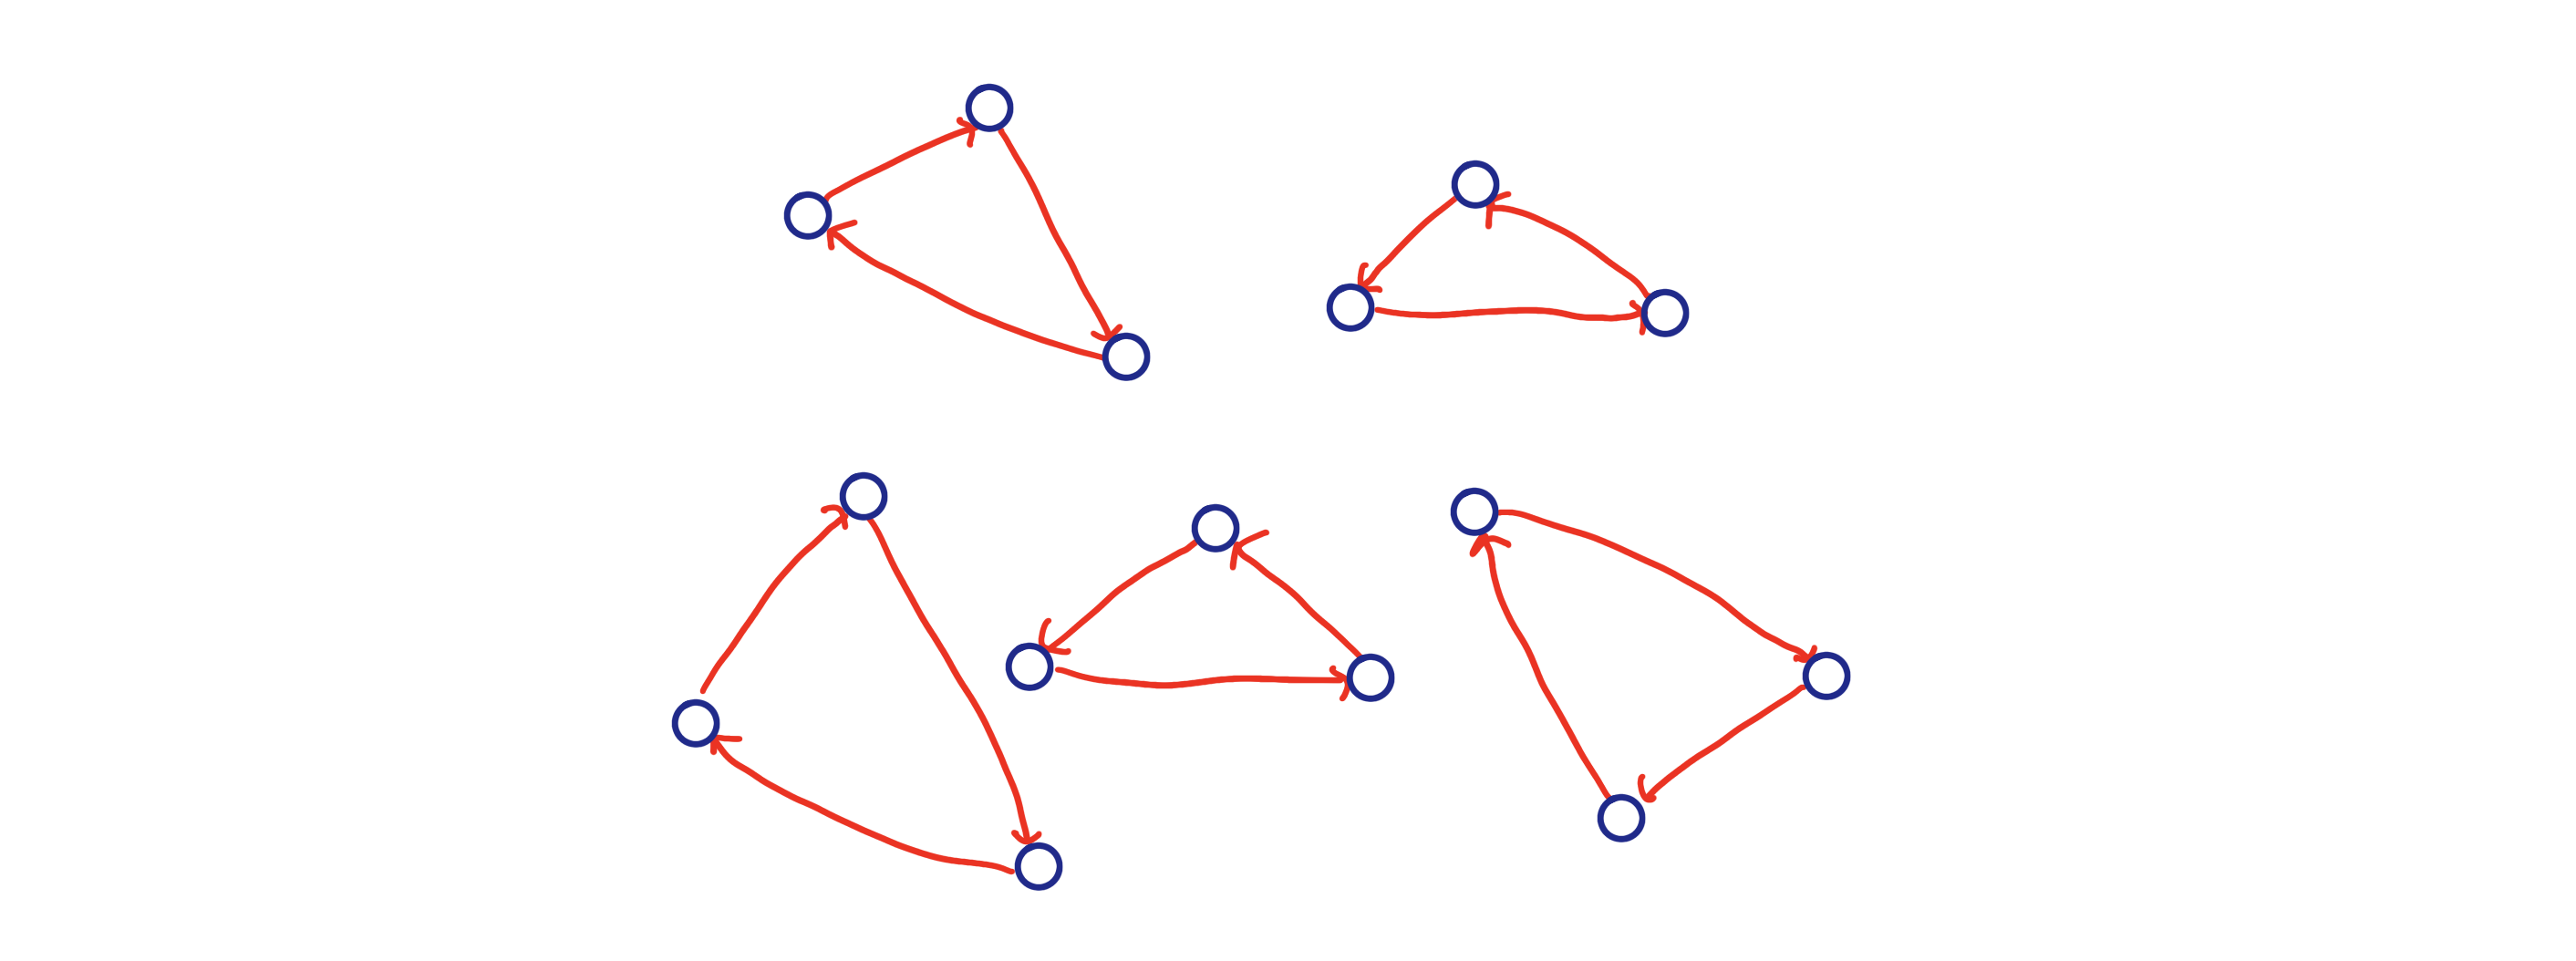
\includegraphics[width=14cm]{final.png}
    \vspace{-0.3cm}
    \caption*{The final strategy}
\end{figure}
\end{document}